\documentclass[a4paper, 12pt]{article}

\usepackage{ctex}
\usepackage{graphicx}
\usepackage{amsmath}
\usepackage{geometry}
\usepackage{mathptmx}
\usepackage[T1]{fontenc}
\usepackage{fancyvrb}
\usepackage{caption}
\usepackage{capt-of}
\usepackage{setspace}

\geometry{left=2.0cm, right=2.0cm, top=2cm, bottom=2cm}   %页边距

\usepackage{tikz}
\usetikzlibrary{graphs, positioning, quotes, shapes.geometric, calc}
% 流程图定义基本形状
\tikzstyle{startstop} = [rectangle, rounded corners, minimum width = 1.6cm, minimum height=0.8cm,text centered, draw = black]
\tikzstyle{io} = [trapezium, trapezium left angle=70, trapezium right angle=110, minimum width=1.6cm, minimum height=0.8cm, text centered, draw=black]
\tikzstyle{process} = [rectangle, minimum width=2.4cm, minimum height=0.8cm, text centered, draw=black]
\tikzstyle{decision} = [diamond, aspect = 3, text centered, draw=black]
% 箭头形式
\tikzstyle{arrow} = [->, ,>=stealth]
\tikzstyle{every node}=[scale=0.7]

\renewcommand{\figurename}{Fig}
\renewcommand{\tablename}{Tab}

\title{\textbf{Report of lab4}}
\author{孟澍 \\ 3210101819}
\date{2022年7月21日}

\begin{document}
\maketitle

\section{Algorithm explanation}
This is the flowchart of my program.

Basic idea: Repeadedly print a line. When interrupt, deal with the interrupt, then continue the program.\\
\begin{figure}[htbp]
  \centering
  \begin{minipage}[t]{0.6\textwidth}
    \centering
    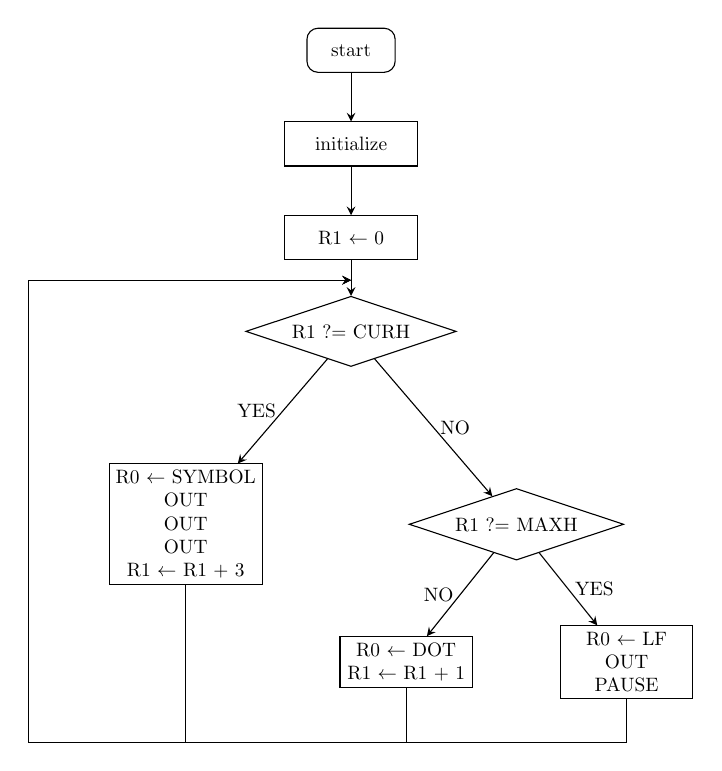
\begin{tikzpicture}[node distance=1.5cm, align=center]
    %定义流程图具体形状
    \node (start) [startstop] {start};
    \node (pro1) [process, below of = start, yshift = -0.2cm] {initialize};
    \node (pro2) [process, below of = pro1, yshift = -0.2cm] {R1 $\leftarrow$ 0};
    \node (dec1) [decision, below of = pro2, yshift = -0.2cm] {R1 ?= CURH};
    \node (pro3) [process, below of = dec1, yshift = -2cm, xshift = -3cm] {R0 $\leftarrow$ SYMBOL \\ OUT \\ OUT \\ OUT \\ R1 $\leftarrow$ R1 + 3};
    \node (dec2) [decision, below of = dec1, yshift = -2cm, xshift = 3cm] {R1 ?= MAXH};
    \node (pro4) [process, below of = dec2, yshift = -1cm, xshift = -2cm] {R0 $\leftarrow$ DOT \\ R1 $\leftarrow$ R1 + 1};
    \node (pro5) [process, below of = dec2, yshift = -1cm, xshift = 2cm] {R0 $\leftarrow$ LF \\ OUT \\ PAUSE};

    %连接具体形状
    \draw [arrow] (start) -- (pro1);
    \draw [arrow] (pro1) -- (pro2);
    \draw [arrow] (pro2) -- (dec1);
    \draw [arrow] (dec1) -- node[anchor = east] {YES} (pro3);
    \draw [arrow] (dec1) -- node[anchor = west] {NO} (dec2);
    \draw [arrow] (dec2) -- node[anchor = east] {NO} (pro4);
    \draw [arrow] (dec2) -- node[anchor = west] {YES} (pro5);

    \draw [arrow] (pro3) -- ($(pro3.south) + (0, -2)$) -- ($(pro3.south) + (-2, -2)$) |- ($(dec1.north) + (0, 0.2)$);
    \draw [arrow] (pro4) |- ($(pro3.south) + (0, -2)$) -- ($(pro3.south) + (-2, -2)$) |- ($(dec1.north) + (0, 0.2)$);
    \draw [arrow] (pro5) |- ($(pro3.south) + (0, -2)$) -- ($(pro3.south) + (-2, -2)$) |- ($(dec1.north) + (0, 0.2)$);
    \end{tikzpicture}
    \captionof{figure}{The flowchart of the program.}
  \end{minipage}%
  \begin{minipage}[t]{0.38\textwidth}
    \centering
    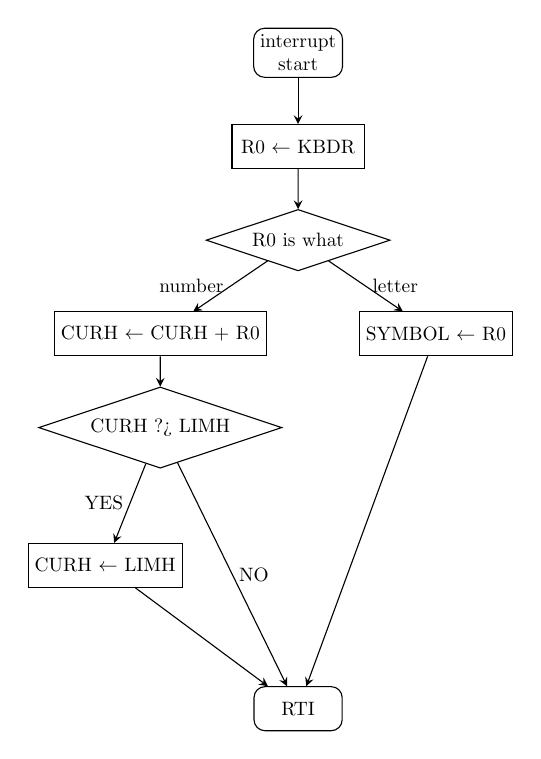
\begin{tikzpicture}[node distance=1.5cm, align=center]
    %定义流程图具体形状
    \node (start) [startstop] {interrupt \\ start};
    \node (pro1) [process, below of = start, yshift = -0.2cm] {R0 $\leftarrow$ KBDR};
    \node (dec1) [decision, below of = pro1, yshift = -0.2cm] {R0 is what};
    \node (pro2) [process, below of = dec1, yshift = -0.2cm, xshift = -2.5cm] {CURH $\leftarrow$ CURH + R0};
    \node (dec2) [decision, below of = pro2, yshift = -0.2cm] {CURH ?> LIMH};
    \node (pro4) [process, below of = dec2, yshift = -1cm, xshift = -1cm] {CURH $\leftarrow$ LIMH};
    \node (pro3) [process, below of = dec1, yshift = -0.2cm, xshift = 2.5cm] {SYMBOL $\leftarrow$ R0};
    \node (stop) [startstop, below of = dec1, yshift = -7cm] {RTI};

    %连接具体形状
    \draw [arrow] (start) -- (pro1);
    \draw [arrow] (pro1) -- (dec1);
    \draw [arrow] (dec1) -- node[anchor = east] {number} (pro2);
    \draw [arrow] (pro2) -- (dec2);
    \draw [arrow] (dec2) -- node[anchor = east] {YES} (pro4);
    \draw [arrow] (dec2) -- node[anchor = west] {NO} (stop);
    \draw [arrow] (dec1) -- node[anchor = west] {letter} (pro3);
    \draw [arrow] (pro3) -- (stop);
    \draw [arrow] (pro4) -- (stop);
    \end{tikzpicture}
    \captionof{figure}{The flowchart of interrupt.}
  \end{minipage}
\end{figure}


\newpage
\section{Source code}
\linespread{0.8}      %行距缩小
\begin{Verbatim}[frame = single, numbers = left, fontsize = \footnotesize]
            .ORIG x0200
            LD R6, OS_SP
            LD R0, USER_PSR
            ADD R6, R6, #-1
            STR R0, R6, #0
            LD R0, USER_PC
            ADD R6, R6, #-1
            STR R0, R6, #0
;
            ; set keyboard to interrupt enable
            LD R0, TEMP
            STI R0, KBSR
            RTI
OS_SP       .FILL x3000
USER_PSR    .FILL x0002
USER_PC     .FILL x3000
KBSR        .FILL xFE00
TEMP        .FILL x4000
            .END
;
;
;
            .ORIG x3000
            ; start of game
START       AND R1, R1, #0
LOOP        LDI R2, PCURH
            NOT R2, R2
            ADD R2, R2 #1
            ADD R2, R2, R1
            BRnp L1
            LDI R0, PSYMBOL
            OUT
            OUT
            OUT
            ADD R1, R1, #3
L1          LD R2, MAXH
            NOT R2, R2
            ADD R2, R2, #1
            ADD R2, R2, R1
            BRn L3
            LD R0, LF
            OUT
            LD R2, PAUSE
L2          ADD R2, R2, #-1
            BRp L2
            LDI R0, PCURH
            BRz START
            ADD R0, R0, #-1
            STI R0, PCURH
            BRnzp START
L3          LD R0, DOT
            OUT
            ADD R1, R1, #1
            BRnzp LOOP
;
MAXH        .FILL x0014
PAUSE       .FILL x3000
DOT         .FILL x002E
LF          .FILL x000A
PCURH       .FILL x3100
PSYMBOL     .FILL x3101
            .END
;
;
;
            .ORIG x3100
CURH        .FILL x0005
SYMBOL      .FILL x0061
            .END
;
;
;
            .ORIG x0180
            .FILL x2000
            .END
;
;
;
            .ORIG x2000
            ; save the values in registers used in interrupt
            ADD R6, R6, #-1
            STR R0, R6, #0
            ADD R6, R6, #-1
            STR R1, R6, #0
;
            LDI R0, KBDR
            LD R1, MAXNUMBER
            NOT R1, R1
            ADD R1, R1, #1
            ADD R1, R1, R0
            BRp LETTER
NUM         LD R1, ZERO             ; is a number
            NOT R1, R1
            ADD R1, R1, #1
            ADD R0, R0, R1
            LDI R1, PPCURH
            ADD R1, R1, R0
            LD R0, LIMH
            NOT R0, R0
            ADD R0, R0, #1
            ADD R0, R0, R1
            BRnz INLIMIT
            LD R1, LIMH
INLIMIT     ADD R1, R1, #1
            STI R1, PPCURH
            BRnzp RETURN
LETTER      STI R0, PPSYMBOL        ; is a letter
            BRnzp RETURN
;
            ; reload the values in registers
RETURN      LDR R1, R6, #0
            ADD R6, R6, #1
            LDR R0, R0, #0
            ADD R6, R6, #1
            RTI
;
ZERO        .FILL x0030
MASK        .FILL xFF00
MAXNUMBER   .FILL x0039
KBSR2       .FILL xFE00
KBDR        .FILL xFE02
PPCURH      .FILL x3100
PPSYMBOL    .FILL x3101
LIMH        .FILL x0011
EMPTY       .FILL xFE00
            .END
\end{Verbatim}
\linespread{0.8}      %行距恢复

\section{Questions TA asked you and your answer in check}

\begin{spacing}{0.8}
\noindent
Question: What's the process of interrupt inside the CPU?\\
Answer: Firsyly, the PSR of the interrupted process is saved in TEMP. Secondly, The processor sets the privilege mode to Supervisor mode (PSR[15]=0). Thirdly, the processor sets the priority level to the priority level of the
interrupting device. Forthly, if the interrupted process is in User mode, R6 is saved in Saved USP and R6 is loaded with the Supervisor Stack Pointer (SSP). Fifthly, TEMP and the PC of the interrupted process are pushed onto the supervisor stack. Sixthly, the interrupting device supplies its eight-bit interrupt vector. Seventhly, the processor expands that vector to the corresponding 16-bit address in the interrupt vector table. Eighthly, The PC is loaded with the contents of memory location that is stored in the interrupt vector. Ninethly, the processor begins execution of the interrupt service routine. Finally, the last instruction executed in an interrupt service routine is RTI. The top two elements of the supervisor stack are popped and loaded into the PC and PSR registers. R6 is loaded with the appropriate stack pointer, depending on the new value of PSR[15]. Processing then continues where the interrupted program left off.
\end{spacing}

\end{document}